\documentclass[11pt,a4paper]{article}
\usepackage[utf8]{inputenc}
\usepackage[spanish]{babel}
\usepackage{amsmath}
\usepackage{amsfonts}
\usepackage{amssymb}
\usepackage{graphicx}
\usepackage{lscape}
\author{Pablo Hernández}
\title{Tarea \#1 Macroeconomía}
\begin{document}
\maketitle

\section*{Ejercicio 3}


\subsection*{a) Obtener datos del INEGI}
Nota metolológica: 

\subsection*{b) Gráficar series de tiempo juntas, en nivles y en logaritmos}


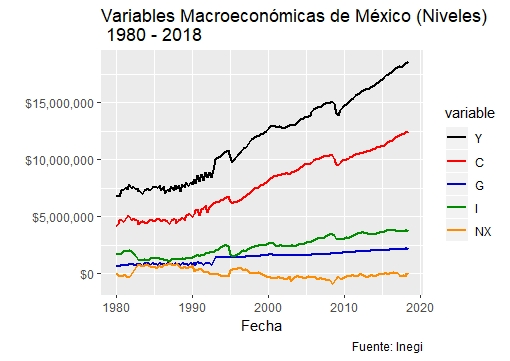
\includegraphics{plotNiveles}
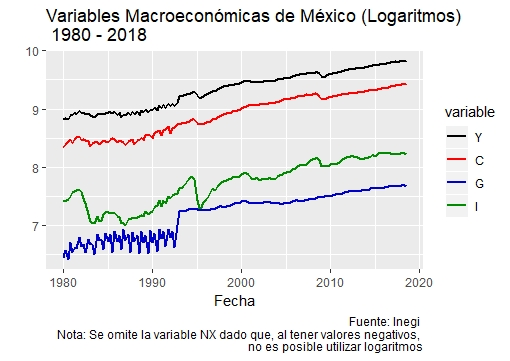
\includegraphics{plotLogs}

\subsection*{c) Gráficar tasas de crecimiento}

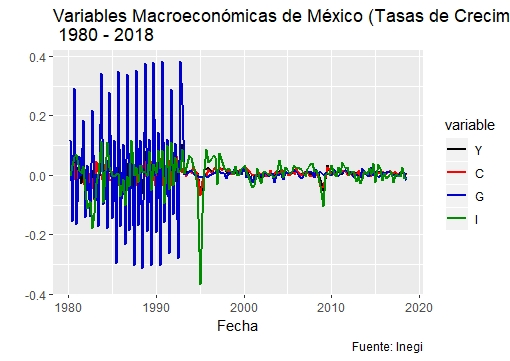
\includegraphics{plotTasas}

\subsection*{d) Gráficar tasas de crecimiento del Ingreso y del Consumo}
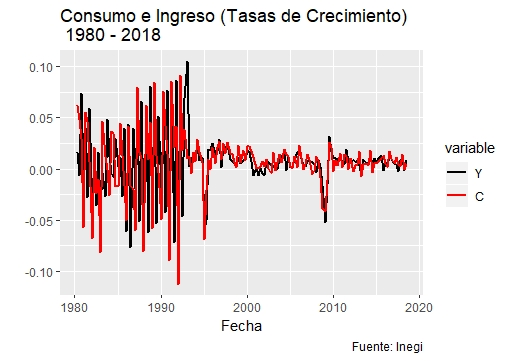
\includegraphics{plotTasas2}


\subsection*{e) Calcular volatilidad de las tasas de crecimiento}


\subsection*{f) Estime cuatro modelos lineales} 
\begin{landscape}
% Table created by stargazer v.5.2.2 by Marek Hlavac, Harvard University. E-mail: hlavac at fas.harvard.edu
% Date and time: vie., feb. 08, 2019 - 12:25:59 p. m.
\begin{table}[!htbp] \centering 
  \caption{Modelos Lineales} 
  \label{} 
\begin{tabular}{@{\extracolsep{5pt}}lcccc} 
\\[-1.8ex]\hline 
\hline \\[-1.8ex] 
 & \multicolumn{4}{c}{\textit{Variable Dependiente}} \\ 
\cline{2-5} 
\\[-1.8ex] & C & \multicolumn{2}{c}{$\vartriangle \% C$} & $lnC$ \\ 
\\[-1.8ex] & (1) & (2) & (3) & (4)\\ 
\hline \\[-1.8ex] 
 $Y_{t}$ & 0.731$^{***}$ &  &  &  \\ 
  & (0.011) &  &  &  \\ 
  & & & & \\ 
 $\vartriangle \% Y_{t}$ &  & 0.549$^{***}$ &  &  \\ 
  &  & (0.061) &  &  \\ 
  & & & & \\ 
 $\vartriangle \% Y_{t-1}$ &  &  & 0.211$^{***}$ &  \\ 
  &  &  & (0.079) &  \\ 
  & & & & \\ 
 $lnY_{t}$ &  &  &  & 1.142$^{***}$ \\ 
  &  &  &  & (0.018) \\ 
  & & & & \\ 
 Constante & $-$961.094$^{***}$ & 0.003$^{***}$ & 0.005$^{***}$ & $-$2.747$^{***}$ \\ 
  & (161.880) & (0.001) & (0.001) & (0.295) \\ 
  & & & & \\ 
\hline \\[-1.8ex] 
Observaciones & 103 & 103 & 102 & 103 \\ 
R$^{2}$ & 0.976 & 0.448 & 0.066 & 0.976 \\ 
R$^{2}$ Ajustada & 0.976 & 0.443 & 0.057 & 0.975 \\ 
Estadístico F & 4,142.973$^{***}$ (gl = 1; 101)  & 82.045$^{***}$ (gl = 1; 101) & 7.108$^{***}$ (gl = 1; 101) & 4,052.524$^{***}$ (gl = 1; 101) \\ 
\hline 
\hline \\[-1.8ex] 
\textit{Nota:}   & \multicolumn {4}{r}{$^{*}$p$<$0.1; $^{**}$p$<$0.05; $^{***}$p$<$0.01} Los estadísticos $t$ se 
muestran entre paréntesis debajo de los coeficientes. \\ 
\end{tabular} 
\end{table} 

\end{landscape}

\subsection{g) Explicación sobre la Hipótesis del Ingreso Permanente}

\end{document}